% ============================================================================
%  SECCIÓN 5.4: DISEÑO DE LA ESTRUCTURA DE PERSISTENCIA
% ============================================================================

\section{Dise~no de la estructura de persistencia}

La estructura de persistencia de la aplicaci\'on \nombreApp{} se dise~na
para garantizar la integridad, seguridad y disponibilidad de los datos.
A continuaci\'on se describe la arquitectura de almacenamiento, las
pol\'iticas de seguridad y el flujo de datos entre los distintos
niveles de persistencia.

\subsection{Arquitectura de niveles}

La persistencia se organiza en tres niveles jer\'arquicos:

\begin{figure}[H]
  \centering
  \caption{Arquitectura de niveles de persistencia}
  \label{fig:arquitectura-persistencia}
  \contenidoConFuente{%
  \begin{tikzpicture}[
    node distance=0.6cm,
    nivel/.style={rectangle, draw=black!60, rounded corners,
      minimum width=5.0cm, minimum height=0.7cm, align=center,
      font=\small},
    flecha/.style={-Stealth, thick}
  ]
    \node[nivel] (ui) {Nivel 1: UI (useState)};
    \node[nivel, below=of ui] (cache)
      {Nivel 2: Cach\'e (React Query)};
    \node[nivel, below=of cache] (server)
      {Nivel 3: Servidor (Supabase)};
    \node[nivel, below=of server] (local)
      {Nivel 4: Local (AsyncStorage)};
    \draw[flecha] (ui) -- (cache);
    \draw[flecha] (cache) -- (server);
    \draw[flecha] (server) -- (local);
  \end{tikzpicture}
  }{Elaboraci\'on propia.}
\end{figure}

\begin{itemize}
  \item \textbf{Nivel 1 (UI):} estado local de React con
    \textit{useState}. Almacena valores temporales de la interfaz
    como filtros, t\'erminos de b\'usqueda y estados de carga.
    Se pierde al cambiar de pantalla.

  \item \textbf{Nivel 2 (Cach\'e):} cach\'e en memoria de React
    Query. Almacena los resultados de las consultas a Supabase
    durante 5 minutos. Se pierde al reiniciar la aplicaci\'on.

  \item \textbf{Nivel 3 (Servidor):} base de datos PostgreSQL
    en Supabase. Almacena todos los datos de dominio de forma
    permanente y centralizada. Persiste entre sesiones y
    dispositivos.

  \item \textbf{Nivel 4 (Local):} almacenamiento local con
    AsyncStorage. Conserva la sesi\'on del usuario (tokens JWT)
    entre aperturas de la aplicaci\'on. Se mantiene hasta que
    el usuario cierre sesi\'on o el token expire.
\end{itemize}

\subsection{Estructura de la base de datos}

La base de datos de Supabase contiene las siguientes tablas
principales:

\begin{table}[H]
  \centering
  \caption{Tablas de la base de datos}
  \contenidoConFuente{%
    \begin{tablaAPA}
      \begin{tabular}{@{}p{3.0cm}p{5.2cm}p{6.6cm}@{}}
        \toprule
        \textbf{Tabla} & \textbf{Campos principales} &
        \textbf{Prop\'osito} \\
        \midrule
        profiles & id, email, full\_name, role,
        created\_at & Perfil de usuario y rol de acceso. \\
        \addlinespace
        scenarios & id, nombre, tipo, descripcion,
        capacidad, direccion, estado &
        Escenarios deportivos del cat\'alogo. \\
        \addlinespace
        scenario\_images & id, scenario\_id,
        storage\_path, url, is\_primary &
        Im\'agenes asociadas a cada escenario. \\
        \addlinespace
        sports & id, nombre, descripcion &
        Deportes disponibles en el sistema. \\
        \addlinespace
        scenario\_sports & scenario\_id, sport\_id &
        Relaci\'on muchos a muchos entre escenarios y
        deportes. \\
        \addlinespace
        events & id, scenario\_id, nombre, fecha,
        hora, descripcion & Eventos pr\'oximos en cada
        escenario. \\
        \addlinespace
        favorites & user\_id, scenario\_id,
        created\_at & Escenarios guardados por el usuario. \\
        \bottomrule
      \end{tabular}
    \end{tablaAPA}%
  }{Elaboraci\'on propia en base a la estructura de la base
  de datos en Supabase.}
\end{table}

\subsection{Diagrama entidad-relaci\'on}

Las relaciones entre las tablas principales se representan en el
siguiente diagrama:

\begin{figure}[H]
  \centering
  \caption{Diagrama entidad-relaci\'on simplificado}
  \label{fig:diagrama-er}
  \contenidoConFuente{%
  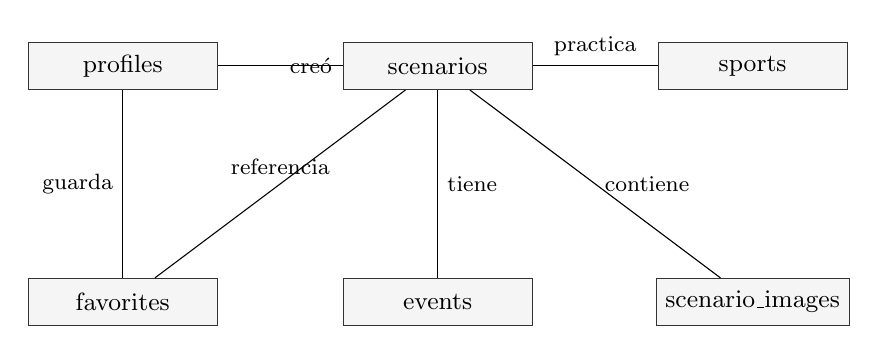
\begin{tikzpicture}[
    entity/.style={rectangle, draw=black!80, fill=gray!8,
      minimum width=2.4cm, minimum height=0.6cm, align=center,
      font=\small},
    rel/.style={diamond, draw=black!60, fill=gray!5,
      minimum width=1.2cm, minimum height=0.5cm, align=center,
      font=\footnotesize},
    line/.style={-}
  ]
    % Entidades
    \node[entity] (profile) at (0, 3) {profiles};
    \node[entity] (scenario) at (4, 3) {scenarios};
    \node[entity] (sport) at (8, 3) {sports};
    \node[entity] (event) at (4, 0) {events};
    \node[entity] (fav) at (0, 0) {favorites};
    \node[entity] (img) at (8, 0) {scenario\_images};

    % Relaciones
    \draw[line] (profile) -- node[right, font=\footnotesize]
      {cre\'o} (scenario);
    \draw[line] (scenario) -- node[above, font=\footnotesize]
      {practica} (sport);
    \draw[line] (scenario) -- node[right, font=\footnotesize]
      {tiene} (event);
    \draw[line] (profile) -- node[left, font=\footnotesize]
      {guarda} (fav);
    \draw[line] (fav) -- node[above, font=\footnotesize]
      {referencia} (scenario);
    \draw[line] (scenario) -- node[right, font=\footnotesize]
      {contiene} (img);
  \end{tikzpicture}
  }{Elaboraci\'on propia.}
\end{figure}

\subsection{Pol\'iticas de seguridad (RLS)}

Las pol\'iticas de seguridad a nivel de fila (Row Level Security)
garantizan que cada usuario solo pueda acceder a los datos que le
corresponden:

\begin{table}[H]
  \centering
  \caption{Pol\'iticas RLS por tabla}
  \contenidoConFuente{%
    \begin{tablaAPA}
      \begin{tabular}{@{}p{2.8cm}p{5.0cm}p{7.4cm}@{}}
        \toprule
        \textbf{Tabla} & \textbf{Pol\'itica} &
        \textbf{Restricci\'on} \\
        \midrule
        profiles & Lectura: p\'ublico &
        Cualquier usuario autenticado puede ver el perfil. \\
        \addlinespace
        scenarios & Lectura: p\'ublico; Escritura:
        gestor+admin &
        Todos leen; solo gestores y admins crean/editan. \\
        \addlinespace
        favorites & CRUD: propietario &
        Solo el usuario propietario puede gestionar sus
        favoritos. \\
        \addlinespace
        events & Lectura: p\'ublico; Escritura:
        gestor+admin; Eliminaci\'on: admin &
        Lectura libre; gestores crean; solo admin elimina. \\
        \addlinespace
        scenario\_images & Lectura: p\'ublico;
        Escritura: admin &
        Solo el admin puede subir o eliminar im\'agenes. \\
        \bottomrule
      \end{tabular}
    \end{tablaAPA}%
  }{Elaboraci\'on propia en base a las migraciones de Supabase.}
\end{table}

\subsection{ \'Indices de optimizaci\'on}

Para mejorar el rendimiento de las consultas m\'as frecuentes, se
crearon \'indices en las columnas utilizadas habitualmente en
cl\'ausulas \textit{WHERE} y \textit{ORDER BY}:

\begin{lstlisting}
-- Catalogo: escenarios activos ordenados por nombre
CREATE INDEX idx_scenarios_estado_nombre
  ON public.scenarios (estado, nombre);

-- Eventos por escenario, ordenados por fecha
CREATE INDEX idx_events_scenario_fecha
  ON public.events (scenario_id, fecha);

-- Favoritos por escenario (para checks RLS)
CREATE INDEX idx_favorites_scenario_id
  ON public.favorites (scenario_id);
\end{lstlisting}

Estos \'indices reducen significativamente el tiempo de respuesta
de las consultas principales de la aplicaci\'on, especialmente
cuando la tabla de escenarios crezca con datos reales.
